\documentclass{article}
\usepackage[dvipnames, table]{xcolor}
\usepackage[utf8]{inputenc}
\usepackage{tabularx}
\usepackage{ltablex}
\usepackage{geometry}
 \geometry{
 a4paper,
 total={170mm,257mm},
 left=27mm,
 top=20mm,
 }
\usepackage{pdfpages}
\title{domainmodel}
\begin{document}
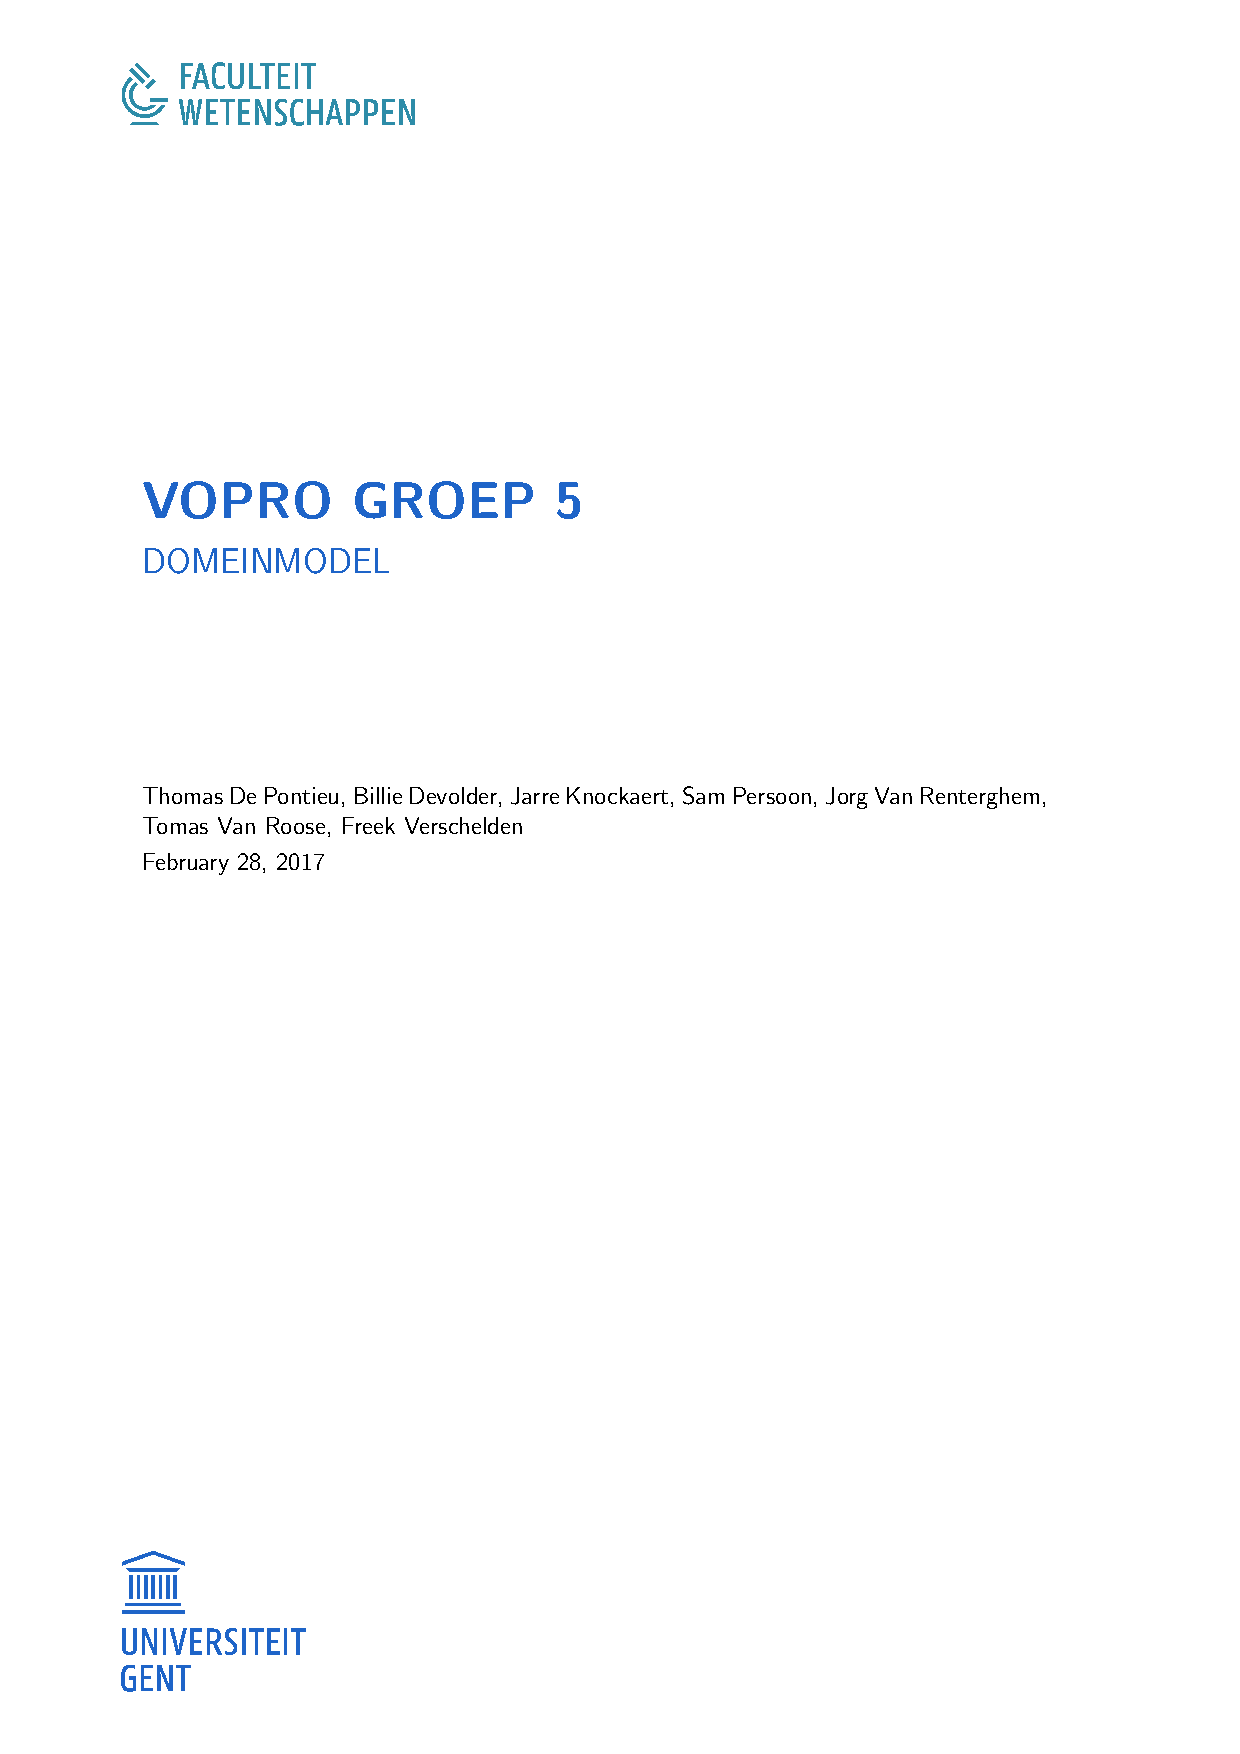
\includepdf[pages={1}]{voorblad_domeinmodel.pdf}
\centering
\rowcolors[]{1}{white}{lightgray}
\begin{tabularx}{\textwidth}{ | l | X |X|} 

\hline
 \multicolumn{3}{| c |}{Domein model}\\

 
 \hline\hline
 Concept & 

 Definitie &
 
 Attributen\\
 \hline\hline
 
 Identiteit & 

 Abstract concept die de gegevens bevat over een (rechts)persoon &
 
 \\
 \hline
 
 Persoon & 

 Een type gebruiker die een persoon voorstelt &
 
 Voornaam\newline
 Achternaam\newline
 Adres\newline
 Functie\newline
 E-mail\newline
 Foto\newline
 Telefoonnummer\newline
 Geboortedatum\\
 \hline
 
 Bedrijf& 

 Een abstract type gebruiker die een bedrijf voorstelt &
 
 Naam\newline
 Adres\newline
 Telefoonnummer\newline
 BTW nummer\newline
 Rekeningnummer\newline
 Vennootschapstype\\
 \hline
 
 Klant & 

 Een klant is een type bedrijf die klant is bij Solvas &
 
 \\
 \hline
 
 Verzekeringsmaatschappij & 

 Een verzekeringsmaatschappij is een type bedrijf dat verzekeringen aanbiedt aan Solvas voor haar klanten &
 \\
 \hline
 
 Leasingmaatschappij & 

 Een leasingmaatschappij is een type bedrijf dat leasing aanbiedt aan de klanten van Solvas &
 \\
 \hline
 
 Account & 

 Concept om in te kunnen loggen  &
 
 Login\newline
 Paswoord\newline
 Rol\\
 \hline
 
 Rol & 

 Bevat rechten om dingen te doen &
 
 Naam\newline
 Rechten\\
 \hline
 
 Vloot & 

 Verzameling van subvloten die tot 1 klant behoren &
 
 Reeks aan subvloten\newline
 Klant\\
 \hline
 
 Subvloot & 

 Een verzameling van voertuigen met 1 bepaald type &
 
 Voertuigtype\newline
 Reeks aan voertuigen\\
 \hline
 
 Voertuig & 

 Bevat de gegevens van een voertuig &
 
 Merk\newline
 Model\newline
 Nummerplaat\newline
 Productiedatum\newline
 Chassisnummer\newline
 Waarde\newline
 Kilometerstand\\
 \hline
 
 Voertuigtype & 

 Bevat type van voertuig &
 
 Type\newline
 Taxatie\\
 \hline
 
 Voertuigverzekeringrelatie & 
 
 Beschrijving van het verband tussen voertuig en verzekering & 
 
 Voertuig\newline
 Verzekering\newline
 Startdatum\newline
 Einddatum\\
 \hline
 
 Verzekering & 

 Abstracte voorstelling van een verzekering &
 
 Verzekeringsmaatschappij\newline
 Prijs\newline
 Franchise\newline
 Berekenmethode\newline
 Waarborgen\\
 \hline
 
 Berekenmethode & 

 Een algoritme om de prijs te berekenen &
 
 \\
 \hline
 
 Waarborg & 
 
 Een garantie van de verzekering  & 
 
 Taksen en lasten\newline
 Commissie\\
 
 \hline
 
 Burgerlijke aanspraakelijkheid & 

 Een type verzekeringswaarborg &
 
 \\
 
 \hline
 Omnium & 

 Een type verzekeringswaarborg &
 
 \\
 \hline
 Rechtsbijstand & 

 Een type verzekeringswaarborg &
 
 \\
 \hline
 
 Veiligheid & 
 
 Een type verzekeringswaarbog &
 
 \\
 \hline
 
 Bijstand & 
 
 Een type verzekeringswaarborg & 
 
 \\
 \hline
 
 Factuur & 

 Abstract concept van uit te voeren betaling of terugstorting &
 
 Ontvanger\newline
 Begunstigde\newline
 Betaler\newline
 Bedrag\newline
 Betaald\newline
 Onderwerp\\
 \hline
 
 Facturatie & 

 Op voorhand vastgelegde kost, subtype van factuur &
 
 Periode\newline
 Startdatum\\
 \hline
 
 Afrekening & 

 Achteraf te betalen of terug te krijgen bedrag &
 
 Periode\newline
 Startdatum\\
 \hline
 
 Correctie & 

 Een subtype van facturatie om correctie door te voeren van een fout in een facturatie of afrekening &
 
 \\
 \hline
 
 Historiek & 

 Lijst van activiteiten &
 
 Lijst van activiteiten\\
 \hline
 
 Activiteit & 

 Een gebeurtenis of wijziging in het systeem, aangebracht door eender wie &
 
 Datum\newline
 Account\newline
 Nieuw object\newline
 Oud object\\
 \hline


\end{tabularx}


\includepdf[pages={3}]{domeinmodel_diagram.pdf}


\end{document}
